\documentclass[tikz,border=6pt]{standalone}
% Shared preamble of the standalone figures: fonts as in the decks, the TikZ
% libraries, the notation, and the styles.
\usepackage[T1]{fontenc}
\usepackage[utf8]{inputenc}
\usepackage[sfdefault,lining]{FiraSans}
\usepackage{FiraMono}
\usepackage{amsmath}
\usetikzlibrary{positioning,arrows.meta,calc,shapes.misc,fit,backgrounds,
                decorations.pathreplacing,patterns,matrix}
% Notation for the MACE4D figures.
%
% Every parameter, symbol, default value, and constant that a figure shows is
% a macro here, so that the figures change from code names to symbols, or
% follow a change of a default, by editing this file alone.
%
%   \codenamestrue   renders each parameter as its code name (current setting)
%   \codenamesfalse  renders the symbolic form
%
% \sym{code name}{symbol} is the switch every parameter macro uses.  A
% parameter that exists on both models carries its owner in code mode.

\newif\ifcodenames
\codenamestrue

\providecommand{\code}[1]{\texttt{#1}}
\newcommand{\sym}[2]{\ifcodenames\code{#1}\else\ensuremath{#2}\fi}
\newcommand{\ctmodel}{\code{ct\_model}}
\newcommand{\macemodel}{\code{MACE4DModel}}
% A key line "code name <-> symbol", shown in code mode only.
\newcommand{\keyline}[2]{\ifcodenames#1~\ensuremath{\leftrightarrow}~\ensuremath{#2}\fi}

% ------------------------------------------------------------ math symbols
% These are always symbolic; the formulas use them, and the key lines tie
% them to the code names.
\newcommand{\symSigY}{\sigma_y}
\newcommand{\symSigProx}{\sigma_p}
\newcommand{\symSigNoise}{\sigma_n}
\newcommand{\symSigX}{\sigma_x}
\newcommand{\symSharpness}{s}
\newcommand{\symBeta}[1]{\beta_{#1}}
\newcommand{\symRho}{\rho}
\newcommand{\symNbrWeightTime}{b_t}
\newcommand{\symNumFrames}{T}
\newcommand{\symFramesPerRotation}{P}
\newcommand{\symOverlap}{f}

% ------------------------------------------------------------------ objects
\newcommand{\frameCube}[1]{\ensuremath{C_{#1}}}          % frame t of the 4D image
\newcommand{\fourD}{\ensuremath{x}}                      % the 4D image
\newcommand{\initImage}{\ensuremath{x^{0}}}              % the initial 4D image
\newcommand{\sinoFrame}[1]{\ensuremath{y_{#1}}}          % the views of frame t
\newcommand{\weightsFrame}[1]{\ensuremath{\Lambda_{#1}}} % the weights of frame t
\newcommand{\projFrame}[1]{\ensuremath{A_{#1}}}          % the frame model
\newcommand{\proxAgent}[1]{\ensuremath{F_{#1}}}          % the prox map of frame t
\newcommand{\dataFitAgent}{\ensuremath{F}}               % all frames' prox maps as one agent
\newcommand{\orientXY}{\sym{XY-t}{\mathrm{XY}t}}
\newcommand{\orientYZ}{\sym{YZ-t}{\mathrm{YZ}t}}
\newcommand{\orientXZ}{\sym{XZ-t}{\mathrm{XZ}t}}
\newcommand{\denoiser}[1]{\ensuremath{G_{#1}}}           % \denoiser{\orientXY}
\newcommand{\stateW}[1]{\ensuremath{W_{#1}}}             % the loop's input to agent k
\newcommand{\outX}[1]{\ensuremath{X_{#1}}}               % the output of agent k
\newcommand{\avgZ}{\ensuremath{z}}
\newcommand{\xbar}{\ensuremath{\bar{x}}}
\newcommand{\filterMatrix}{\sym{filter\_matrix}{H}}
\newcommand{\genInit}{\code{'init'}}                     % the generator of the partitions
\newcommand{\genIteration}{the iteration number}          % the generator of the subset order

% --------------------------------------------- parameters and their defaults
% Scan and frames (constructor arguments of MACE4DModel)
\newcommand{\pFramesPerRotation}{\sym{frames\_per\_rotation}{\symFramesPerRotation}}
\newcommand{\defFramesPerRotation}{6}
\newcommand{\pFrameOverlapFactor}{\sym{frame\_overlap\_factor}{\symOverlap}}
\newcommand{\defFrameOverlapFactor}{2.0}
\newcommand{\pNumFrames}{\sym{num\_frames}{\symNumFrames}}
\newcommand{\defNumFrames}{all}

% Set on ct_model; reach the frame models
\newcommand{\pSnrDb}{\sym{snr\_db}{\mathrm{SNR}_{\mathrm{dB}}}}
\newcommand{\defSnrDb}{30}
\newcommand{\pSharpnessCt}{\sym{ct\_model.sharpness}{\symSharpness_{\mathrm{ct}}}}
\newcommand{\defSharpnessCt}{1.0}
\newcommand{\pSigmaProxCt}{\sym{ct\_model.sigma\_prox}{\symSigProx^{\mathrm{ct}}}}
\newcommand{\pSigmaXCt}{\sym{ct\_model.sigma\_x}{\symSigX^{\mathrm{ct}}}}
\newcommand{\pPQTCt}{\sym{ct\_model.p, q, T}{(p, q, T)_{\mathrm{ct}}}}
\newcommand{\pSigmaY}{\sym{sigma\_y}{\symSigY}}

% Set on MACE4DModel
\newcommand{\pSigmaProxMace}{\sym{MACE4DModel.sigma\_prox}{\symSigProx}}
\newcommand{\defSigmaProxMace}{None (estimated per frame)}
\newcommand{\pSigmaNoise}{\sym{sigma\_noise}{\symSigNoise}}
\newcommand{\defSigmaNoise}{None (estimated)}
\newcommand{\pSigmaXMace}{\sym{MACE4DModel.sigma\_x}{\symSigX}}
\newcommand{\defSigmaXMace}{estimated}
\newcommand{\pSharpnessMace}{\sym{MACE4DModel.sharpness}{\symSharpness}}
\newcommand{\defSharpnessMace}{0.0}
\newcommand{\pPQTMace}{\sym{MACE4DModel.p, q, T}{(p, q, T)}}
\newcommand{\defPQT}{2.0, 1.2, 1.0}
\newcommand{\pNbrWeightTime}{\sym{nbr\_weight\_time}{\symNbrWeightTime}}
\newcommand{\defNbrWeightTime}{1.0}
\newcommand{\pMacePriorWeight}{\sym{mace\_prior\_weight}{\beta}}
\newcommand{\defMacePriorWeight}{0.5}
\newcommand{\pRhoMann}{\sym{rho\_mann}{\symRho}}
\newcommand{\defRhoMann}{0.5}
\newcommand{\pProxNumIterations}{\sym{prox\_num\_iterations}{N_p}}
\newcommand{\defProxNumIterations}{3}
\newcommand{\pProxPartitionAdvance}{\sym{prox\_partition\_advance}{a}}
\newcommand{\defProxPartitionAdvance}{1.0}
\newcommand{\pProxWarmStart}{\code{prox\_warm\_start}}
\newcommand{\defProxWarmStart}{True}
\newcommand{\pProxStopThreshold}{\code{prox\_stop\_threshold}}
\newcommand{\defProxStopThreshold}{0.02}
\newcommand{\pDenoiserWarmStart}{\code{denoiser\_warm\_start}}
\newcommand{\defDenoiserWarmStart}{False}
\newcommand{\pDenoiseSlabGb}{\code{denoise\_slab\_gb}}
\newcommand{\defDenoiseSlabGb}{2.0}
\newcommand{\pDejitter}{\code{dejitter}}
\newcommand{\defDejitter}{True}
\newcommand{\pDevicePool}{\code{set\_device\_pool}}
\newcommand{\pNumDevicesEnv}{\code{MBIRTORCH\_NUM\_DEVICES}}

% Arguments of MACE4DModel.recon
\newcommand{\pMaxIterations}{\sym{max\_iterations}{N}}
\newcommand{\defMaxIterations}{10}
\newcommand{\pStopThreshold}{\code{stop\_threshold\_change\_pct}}
\newcommand{\defStopThreshold}{0.2}
\newcommand{\pSeed}{\code{seed}}
\newcommand{\defSeed}{None}
\newcommand{\pInitRecon}{\code{init\_recon}}
\newcommand{\pInitDir}{\code{init\_dir}}

% ---------------------------------------------------------------- constants
\newcommand{\cInitIterations}{15}        % iterations of the per-frame initial image
\newcommand{\cDenoiseMaxIterations}{15}  % iterations per denoised volume, at most
\newcommand{\cDenoiseStopPct}{0.05}      % percent change that stops a denoised volume
\newcommand{\cSigmaXFactor}{0.2}         % sigma_x and sigma_prox estimates: factor * 2^sharpness * std
\newcommand{\cSigmaXFloor}{10^{-6}}      % floor of the denoiser sigma_x estimate
\newcommand{\cSigmaXBase}{1.0}           % base default of sigma_x when no estimate runs
\newcommand{\cDenoiseSubsets}{16}        % pixel subsets of a denoiser partition, at most
\newcommand{\cPixelsPerSubset}{64}       % fewer pixels per subset than this and the count drops

% ------------------------------------------- symbols the figures use inline
\newcommand{\symPriorWeight}{\ensuremath{w}}    % the value of the prior weight
\newcommand{\symFilterMatrix}{\ensuremath{H}}   % the temporal filter
\newcommand{\symFrameIndex}{\ensuremath{t}}
\newcommand{\symNumDevices}{\ensuremath{n}}     % the size of the device pool
\newcommand{\degsym}{\ensuremath{^{\circ}}}
% Argument values of the device pool selector
\newcommand{\valNone}{\code{None}}
\newcommand{\valCpu}{\code{'cpu'}}
\newcommand{\valGpu}{\code{'gpu'}}
% Derived defaults, in degrees (integers; add rounding if a default ever gives a fraction)
\newcommand{\defFrameStepDeg}{\pgfmathparse{int(360/\defFramesPerRotation)}\pgfmathresult}
\newcommand{\defFrameSpanDeg}{\pgfmathparse{int(\defFrameOverlapFactor*360/\defFramesPerRotation)}\pgfmathresult}
% Axis labels of the 4D image
\newcommand{\axisT}{\ensuremath{t}}
\newcommand{\axisX}{\ensuremath{x}}
\newcommand{\axisY}{\ensuremath{y}}
\newcommand{\axisZ}{\ensuremath{z}}

% Colors and TikZ styles shared by the MACE4D figures.
%
% Blue is the data-fit side, green the priors, amber the consensus state.
% A solid arrow carries a value the user set; a dashed arrow carries an
% estimate.  \cube draws one frame of the 4D image.

\definecolor{datafitBlue}{HTML}{3D6B99}
\definecolor{priorGreen}{HTML}{2E7D32}
\definecolor{stateAmber}{HTML}{B26B1F}
\definecolor{warnRed}{HTML}{A23B3B}
\definecolor{inkGray}{HTML}{5A5A5A}
\definecolor{lineGray}{HTML}{9A9A9A}
\definecolor{paleBlue}{HTML}{E3ECF5}
\definecolor{paleGreen}{HTML}{E4F0E4}
\definecolor{paleAmber}{HTML}{F5EBDD}
\definecolor{paleGray}{HTML}{F0F0F0}

\tikzset{
  every node/.style={font=\small},
  box/.style={draw, rounded corners=3pt, thick, align=center, inner sep=5pt,
              minimum height=8mm},
  datafit/.style={box, draw=datafitBlue, fill=paleBlue},
  prior/.style={box, draw=priorGreen, fill=paleGreen},
  state/.style={box, draw=stateAmber, fill=paleAmber},
  plain/.style={box, draw=lineGray, fill=paleGray},
  note/.style={font=\footnotesize, text=inkGray, align=left},
  notebox/.style={note, draw=lineGray, rounded corners=2pt, inner sep=4pt,
                  fill=white},
  param/.style={font=\footnotesize, align=left},
  title/.style={font=\bfseries, align=left},
  setarrow/.style={-{Stealth[length=2mm]}, thick},
  estarrow/.style={-{Stealth[length=2mm]}, thick, dashed, inkGray},
  flow/.style={-{Stealth[length=2mm]}, semithick},
  flowblue/.style={flow, datafitBlue},
  flowgreen/.style={flow, priorGreen},
  flowamber/.style={flow, stateAmber},
  cut/.style={-{Stealth[length=1.5mm]}, thin, inkGray},
  cubeFront/.style={fill=white, draw=black!70, thin},
  cubeTop/.style={fill=black!8, draw=black!70, thin},
  cubeSide/.style={fill=black!20, draw=black!70, thin},
}

% \cube{x}{y}{size}{label}: a cube whose front face has its lower left
% corner at (x, y) and side length size, with a label on the front face.
\newcommand{\cube}[4]{%
  \begin{scope}[shift={(#1,#2)}]
    \pgfmathsetmacro{\cubeDepth}{0.35*#3}
    \draw[cubeTop] (0,#3) -- (\cubeDepth,#3+\cubeDepth) -- (#3+\cubeDepth,#3+\cubeDepth) -- (#3,#3) -- cycle;
    \draw[cubeSide] (#3,0) -- (#3+\cubeDepth,\cubeDepth) -- (#3+\cubeDepth,#3+\cubeDepth) -- (#3,#3) -- cycle;
    \draw[cubeFront] (0,0) rectangle (#3,#3);
    \node at (0.5*#3,0.5*#3) {#4};
  \end{scope}}

% \arrowkey{x}{y}: the legend of the two arrow kinds, anchored at (x, y).
\newcommand{\arrowkey}[2]{%
  \draw[setarrow] (#1,#2) -- ++(1,0) node[note, right] {set by the user};
  \draw[estarrow] (#1,#2-0.45) -- ++(1,0) node[note, right] {estimated from the data};}


\usepackage{array}
\hyphenpenalty=10000
\exhyphenpenalty=10000

% Drawing helpers: a thin cut plane through the cube whose front face has its
% lower left corner at (x, y) and side length s.
% \plateZ: a plane at one z index.  \plateX: a plane at one x index.
% \plateY: a plane at one y index.
\newcommand{\plateZ}[3]{%
  \begin{scope}[shift={(#1,#2)}]
    \pgfmathsetmacro{\plD}{0.35*#3}
    \pgfmathsetmacro{\plE}{0.15*#3}
    \pgfmathsetmacro{\plH}{0.34*#3}
    \filldraw[priorGreen, fill opacity=0.40, thin]
      (-\plE,\plH) -- (#3+\plE,\plH) -- (#3+\plE+\plD,\plH+\plD) -- (-\plE+\plD,\plH+\plD) -- cycle;
  \end{scope}}
\newcommand{\plateX}[3]{%
  \begin{scope}[shift={(#1,#2)}]
    \pgfmathsetmacro{\plD}{0.35*#3}
    \pgfmathsetmacro{\plE}{0.15*#3}
    \pgfmathsetmacro{\plC}{0.38*#3}
    \filldraw[priorGreen, fill opacity=0.40, thin]
      (\plC,-\plE) -- (\plC+\plD,-\plE+\plD) -- (\plC+\plD,#3+\plE+\plD) -- (\plC,#3+\plE) -- cycle;
  \end{scope}}
\newcommand{\plateY}[3]{%
  \begin{scope}[shift={(#1,#2)}]
    \pgfmathsetmacro{\plD}{0.35*#3}
    \pgfmathsetmacro{\plA}{0.5*\plD}
    \filldraw[priorGreen, fill opacity=0.40, thin]
      (\plA,\plA) rectangle (\plA+#3,\plA+#3);
  \end{scope}}

\begin{document}
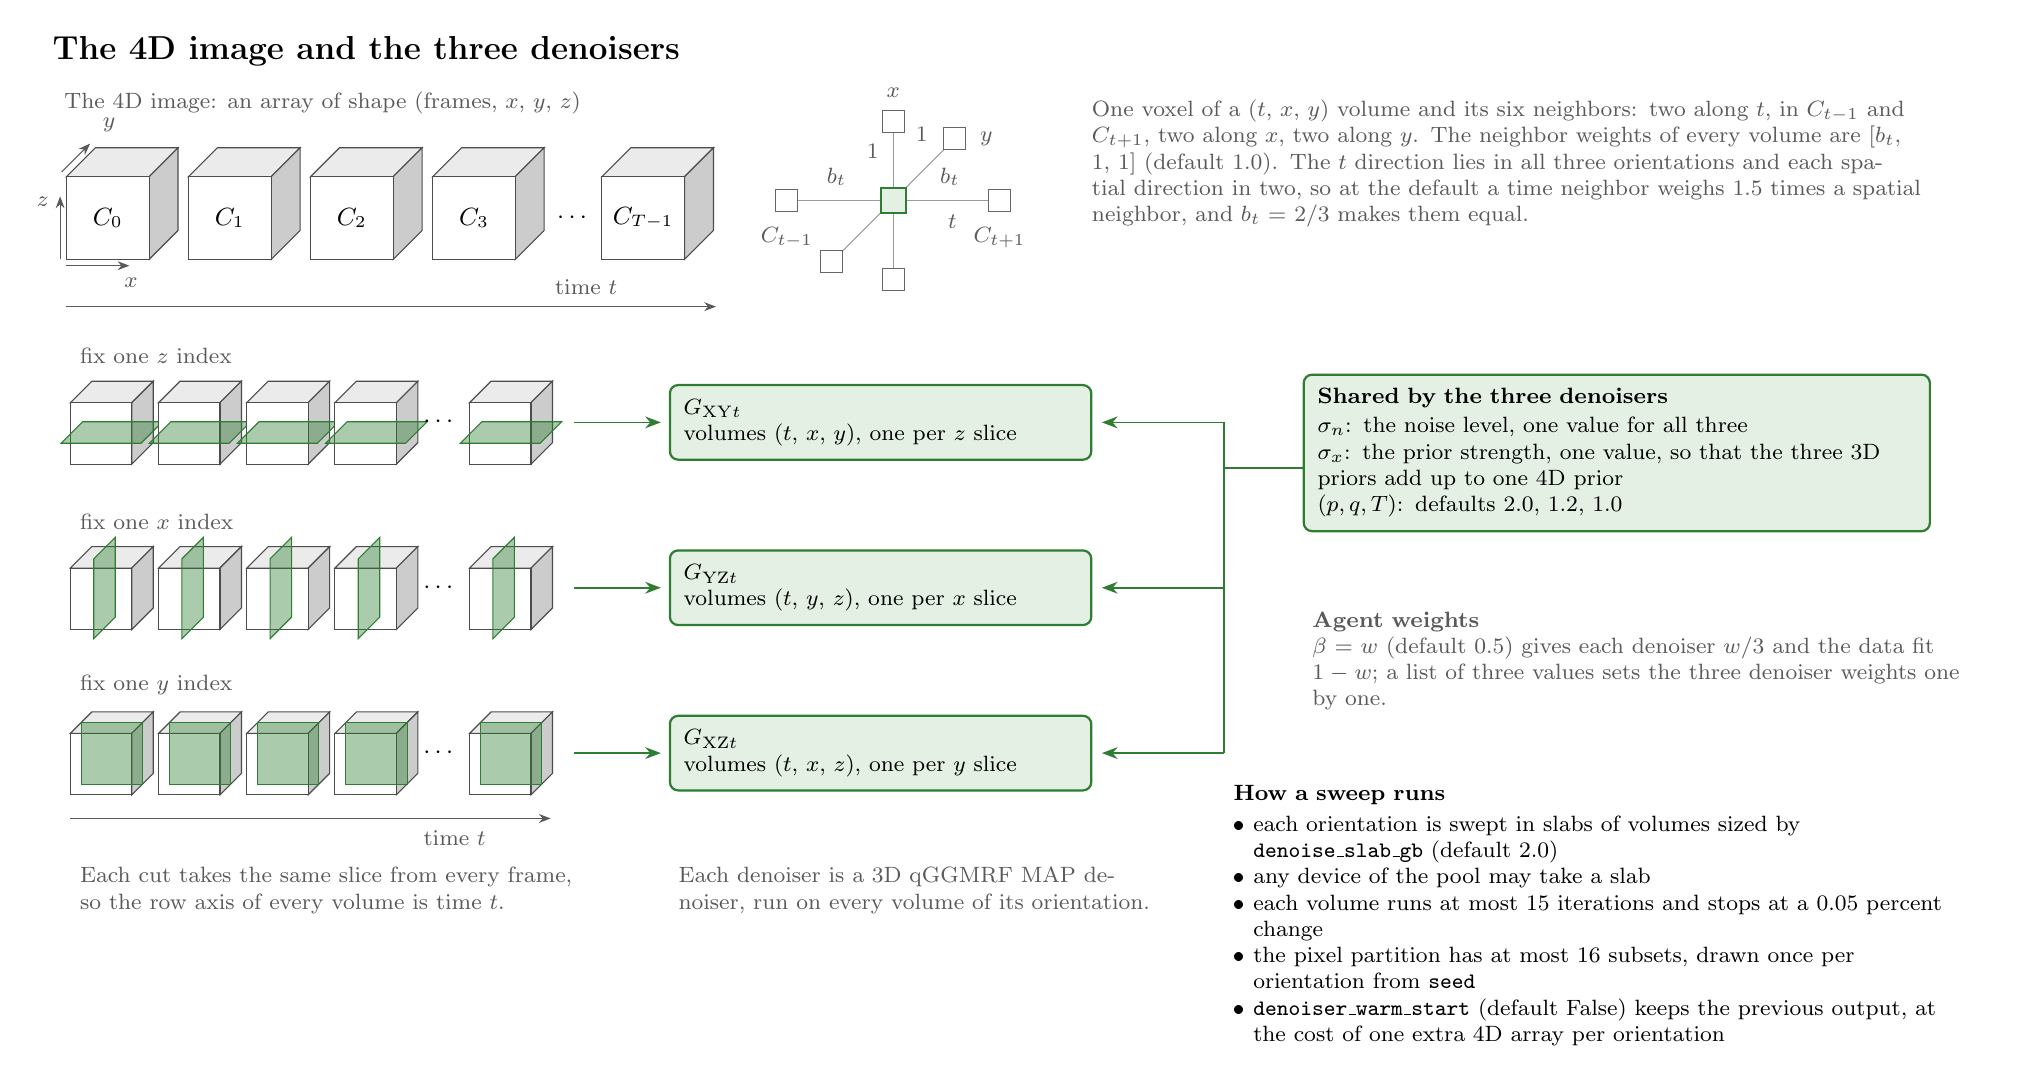
\begin{tikzpicture}

% ---------------------------------------------------------------- the title
\node[title, font=\large\bfseries, anchor=north west] at (0.2,13.9)
  {The 4D image and the three denoisers};

% ------------------------------------------------- the 4D image: one row of
% frames, with the axes marked on the first frame and time along the row
\node[note, anchor=north west] at (0.35,13.2)
  {The 4D image: an array of shape (frames, \axisX, \axisY, \axisZ)};
\cube{0.50}{10.95}{1.05}{\frameCube{0}}
\cube{2.05}{10.95}{1.05}{\frameCube{1}}
\cube{3.60}{10.95}{1.05}{\frameCube{2}}
\cube{5.15}{10.95}{1.05}{\frameCube{3}}
\node at (6.95,11.48) {\ensuremath{\cdots}};
\cube{7.30}{10.95}{1.05}{\frameCube{\symNumFrames-1}}
\draw[cut] (0.50,10.87) -- (1.30,10.87);
\node[note, anchor=north] at (1.32,10.84) {\axisX};
\draw[cut] (0.42,10.95) -- (0.42,11.75);
\node[note, anchor=east] at (0.40,11.68) {\axisZ};
\draw[cut] (0.44,12.06) -- (0.80,12.42);
\node[note, anchor=south west] at (0.84,12.44) {\axisY};
\draw[cut] (0.50,10.35) -- (8.75,10.35)
  node[note, above=1pt, pos=0.80] {time \axisT};

% ------------------------------- the inset: one voxel and its six neighbors
\begin{scope}[shift={(11.0,11.70)}]
  \foreach \nx/\ny in {-1.35/0, 1.35/0, 0/1.00, 0/-1.00, 0.78/0.78, -0.78/-0.78}
    {\draw[lineGray, thin] (0,0) -- (\nx,\ny);
     \draw[fill=white, draw=black!60, thin] (\nx-0.14,\ny-0.14) rectangle (\nx+0.14,\ny+0.14);}
  \draw[fill=paleGreen, draw=priorGreen, thick] (-0.16,-0.16) rectangle (0.16,0.16);
  \node[note, anchor=south] at (-0.72,0.06) {\ensuremath{\symNbrWeightTime}};
  \node[note, anchor=south] at (0.72,0.06) {\ensuremath{\symNbrWeightTime}};
  \node[note, anchor=east] at (-0.06,0.62) {1};
  \node[note, anchor=south east] at (0.56,0.62) {1};
  \node[note, anchor=north] at (-1.35,-0.22) {\frameCube{\axisT-1}};
  \node[note, anchor=north] at (1.35,-0.22) {\frameCube{\axisT+1}};
  \node[note, anchor=south] at (0,1.18) {\axisX};
  \node[note, anchor=west] at (0.98,0.78) {\axisY};
  \node[note, anchor=north] at (0.75,-0.06) {\axisT};
\end{scope}
\node[note, anchor=north west, text width=10.6cm] at (13.4,13.1)
  {One voxel of a (\axisT, \axisX, \axisY) volume and its six neighbors: two
   along \axisT, in \frameCube{\axisT-1} and \frameCube{\axisT+1}, two along
   \axisX, two along \axisY. The neighbor weights of every volume are
   [\pNbrWeightTime, 1, 1] (default \defNbrWeightTime). The \axisT{} direction
   lies in all three orientations and each spatial direction in two, so at the
   default a time neighbor weighs 1.5 times a spatial neighbor, and
   \pNbrWeightTime{} = 2/3 makes them equal.};

% --------------------------------- the three cuts: one row of frames each,
% a thin plane through every frame, and an arrow to the denoiser of that cut
\node[note, anchor=south west] at (0.55,9.50) {fix one \axisZ{} index};
\foreach \i in {0,1,2,3}
  {\pgfmathsetmacro{\xx}{0.55+1.12*\i}
   \cube{\xx}{8.35}{0.78}{}\plateZ{\xx}{8.35}{0.78}}
\node at (5.25,8.88) {\ensuremath{\cdots}};
\cube{5.62}{8.35}{0.78}{}\plateZ{5.62}{8.35}{0.78}
\draw[flowgreen] (6.95,8.88) -- (8.05,8.88);

\node[note, anchor=south west] at (0.55,7.40) {fix one \axisX{} index};
\foreach \i in {0,1,2,3}
  {\pgfmathsetmacro{\xx}{0.55+1.12*\i}
   \cube{\xx}{6.25}{0.78}{}\plateX{\xx}{6.25}{0.78}}
\node at (5.25,6.78) {\ensuremath{\cdots}};
\cube{5.62}{6.25}{0.78}{}\plateX{5.62}{6.25}{0.78}
\draw[flowgreen] (6.95,6.78) -- (8.05,6.78);

\node[note, anchor=south west] at (0.55,5.30) {fix one \axisY{} index};
\foreach \i in {0,1,2,3}
  {\pgfmathsetmacro{\xx}{0.55+1.12*\i}
   \cube{\xx}{4.15}{0.78}{}\plateY{\xx}{4.15}{0.78}}
\node at (5.25,4.68) {\ensuremath{\cdots}};
\cube{5.62}{4.15}{0.78}{}\plateY{5.62}{4.15}{0.78}
\draw[flowgreen] (6.95,4.68) -- (8.05,4.68);

\draw[cut] (0.55,3.85) -- (6.65,3.85)
  node[note, below=1pt, pos=0.80] {time \axisT};
\node[note, anchor=north west, text width=6.4cm] at (0.55,3.35)
  {Each cut takes the same slice from every frame, so the row axis of every
   volume is time \axisT.};

% ------------------------------------------------------ the three denoisers
\node[prior, font=\footnotesize, align=left, text width=5.0cm, anchor=west]
  at (8.15,8.88) {\denoiser{\orientXY}\\ volumes (\axisT, \axisX, \axisY), one per \axisZ{} slice};
\node[prior, font=\footnotesize, align=left, text width=5.0cm, anchor=west]
  at (8.15,6.78) {\denoiser{\orientYZ}\\ volumes (\axisT, \axisY, \axisZ), one per \axisX{} slice};
\node[prior, font=\footnotesize, align=left, text width=5.0cm, anchor=west]
  at (8.15,4.68) {\denoiser{\orientXZ}\\ volumes (\axisT, \axisX, \axisZ), one per \axisY{} slice};
\node[note, anchor=north west, text width=6.2cm] at (8.15,3.35)
  {Each denoiser is a 3D qGGMRF MAP denoiser, run on every volume of its
   orientation.};

% ------------------------- the parameters the three denoisers share, fed to
% each of them
\node[prior, font=\footnotesize, align=left, text width=7.6cm, anchor=north west]
  at (16.2,9.50)
  {{\bfseries Shared by the three denoisers}\\[1pt]
   \pSigmaNoise{}: the noise level, one value for all three\\
   \pSigmaXMace{}: the prior strength, one value, so that the three 3D priors
   add up to one 4D prior\\
   \pPQTMace{}: defaults \defPQT};
\draw[priorGreen, semithick] (16.2,8.30) -- (15.20,8.30);
\draw[priorGreen, semithick] (15.20,8.88) -- (15.20,4.68);
\foreach \y in {8.88,6.78,4.68} \draw[flowgreen] (15.20,\y) -- (13.65,\y);

% ------------------------------------------------- the weight of each agent
\node[note, anchor=north west, text width=8.4cm] at (16.2,6.60)
  {{\bfseries Agent weights}\\
   \pMacePriorWeight{} = \symPriorWeight{} (default \defMacePriorWeight)
   gives each denoiser \ensuremath{\symPriorWeight/3} and the data fit
   \ensuremath{1 - \symPriorWeight}; a list of three values sets the three
   denoiser weights one by one.};

% ------------------------------------------------------- how a sweep is run
\node[param, anchor=north west, text width=9.5cm] at (15.20,4.40)
  {{\bfseries How a sweep runs}\\[2pt]
   \begin{tabular}{@{}l@{~}>{\raggedright\arraybackslash}p{9.0cm}@{}}
     \textbullet & each orientation is swept in slabs of volumes sized by
       \pDenoiseSlabGb{} (default \defDenoiseSlabGb)\\
     \textbullet & any device of the pool may take a slab\\
     \textbullet & each volume runs at most \cDenoiseMaxIterations{} iterations
       and stops at a \cDenoiseStopPct{} percent change\\
     \textbullet & the pixel partition has at most \cDenoiseSubsets{} subsets,
       drawn once per orientation from \pSeed\\
     \textbullet & \pDenoiserWarmStart{} (default \defDenoiserWarmStart) keeps
       the previous output, at the cost of one extra 4D array per orientation
   \end{tabular}};

% ------------------------------------------ the code names and their symbols
\ifcodenames
  \node[notebox, anchor=north west, text width=8.6cm] at (0.55,2.30)
    {\keyline{\pSigmaNoise}{\symSigNoise} \hfill
     \keyline{\pSigmaXMace}{\symSigX}\\
     \keyline{\pNbrWeightTime}{\symNbrWeightTime} \hfill
     \keyline{\pMacePriorWeight}{\symBeta{k}}};
\fi

\end{tikzpicture}
\end{document}
